\documentclass[compress]{beamer}
\mode<presentation>
{
 \usetheme{Vilanova}
}

\usepackage[french]{babel}

\usepackage[utf8]{inputenc}

\usepackage{times}
\usepackage[T1]{fontenc}

\usepackage{amsfonts}
\usepackage{amsmath}
\usepackage{amssymb}
\usepackage{tikz}
\usepackage{eurosym}
%\usepackage{url}
\usepackage[normal]{subfigure}
\newcommand{\goodgap}{%
	\hspace{\subfigtopskip}%
	\hspace{\subfigbottomskip}}



%\newtheorem{definition}{Definition}

\title{Extraction de primitives}




\author
{jordi.inglada@cesbio.cnes.fr}
\normalsize

\institute[Cesbio] % (optional, but mostly needed)
{\textsc{Centre d'Études Spatiales de la Biosphère, Toulouse, France}}

\date{}

\pgfdeclareimage[height=96mm,width=128mm]{background}{fondsClairSansLogo}
\setbeamertemplate{background}{\pgfuseimage{background}}
\pgfdeclareimage[height=0.6cm]{logoIncrust}{logoIncrust}
\pgfdeclareimage[height=0.5cm]{logo_cesbio}{logo_cesbio}
\logo{
\begin{tabular}{lp{0.25\textwidth}lp{0.25\textwidth}r}
\href{http://www.cesbio.ups-tlse.fr/}{\pgfuseimage{logo_cesbio}}
&&\footnotesize{AUF - Marrakech 2011}&&
\href{http://www.orfeo-toolbox.org}{\pgfuseimage{logoIncrust}}\\
\end{tabular}
}


\subject{Extraction de primitives}




% Delete this, if you do not want the table of contents to pop up at
% the beginning of each subsection:
\AtBeginSubsection[]
{
  \begin{frame}<beamer>
    \frametitle{Outline}
    \tableofcontents[currentsection,currentsubsection]
  \end{frame}
}




% If you wish to uncover everything in a step-wise fashion, uncomment
% the following command: 

%\beamerdefaultoverlayspecification{<+->}
\begin{document}

\begin{frame}
  \titlepage
  \begin{center}
{\tiny Ce contenu est dérivé de la formation \href{http://www.orfeo-toolbox.org/packages/PragmaticRemoteSensing-handout.pdf}{``Pragmatic Remote
  Sensing''} dispensée par J. Inglada et E. Christophe en juillet 2010
  dans le cadre du colloque IGARSS. Il est mis à disposition selon les termes de la licence :\\
Creative Commons Paternité – Partage à l’Identique 3.0 non transcrit.} \href{http://creativecommons.org/licenses/by-sa/3.0/}{
\includegraphics[width=0.05\textwidth]{/home/inglada/Dev/GH/IGARSS2010/Tutorial/Slides/Ressources/CC-licence.png}}    
  \end{center}
\end{frame}


\section[Intro]{La classification d'images}
\begin{frame}
\frametitle{La classification d'images}
  \begin{itemize}
  \item Définition : procédure par laquelle on attibue une étiquette
    aux objets (pixels de l'image)
  \item Supervisée
  \item Non-supervisée
  \item Orientée pixel
  \item Orientée objet
  \end{itemize}
\end{frame}

\begin{frame}
  \frametitle{Données pour la classification}
  \begin{itemize}
  \item Images (réflectances)
  \item Primitives
    \begin{itemize}
    \item Indices radiométriques: NDVI, brillance, couleur, angle
      spectral, etc.
    \item Statistiques, textures, etc.
    \item Transformatiosn: ACP, MNF, ondelettes, etc.
    \end{itemize}
  \item Données exogènes
    \begin{itemize}
    \item MNT, cartes, etc.
    \end{itemize}
  \end{itemize}
\end{frame}

\begin{frame}
  \frametitle{La classification en 4 étapes}
  \begin{itemize}
  \item Sélection des attributs pertinents (primitives, etc.)
  \item Création d'un vecteur d'attributs par pixel
  \item Choix de l'étiquette de la classe (dans le cas supervisé)
  \item Apprentissage du classifieur
  \end{itemize}
\end{frame}
\section[Non-supervisé]{Classification non-supervisée}
\label{sec:unsupervised}
\begin{frame}
\frametitle{Classification non-supervisée}
  \begin{itemize}
  \item Aussi appelée {\em clustering}
  \item Nécessite une interprétation des résultats (reconnaissance des
    classes)
    \begin{itemize}
    \item Les étiquettes des classes sont des nombres (1, 2, ...)
    \end{itemize}
  \item Pas besoin de vérité terrain ou d'exemples
    \begin{itemize}
    \item Le nombre de classes est souvent choisi à la main
    \item Autres paramètres sont aussi nécessaires
    \end{itemize}
  \item Exemples: k-moyennes, ISO-Data, carte de Kohonen
  \end{itemize}
\end{frame}

\begin{frame}
  \frametitle{Exemple: K-moyenens}
\setbeamercovered{invisible}

{\tiny
  \begin{center}
    \begin{tabular}{lc}
     \onslide<2->{1. les k ``moyennes'' initiales sont} &\\
\onslide<2->{choisies aléatoirement.}&\\
&\onslide<2->{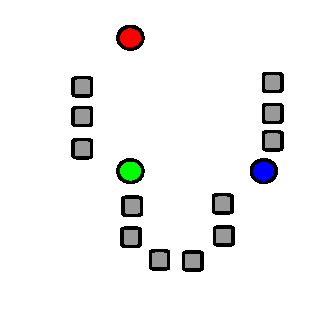
\includegraphics[width=0.15\textwidth]{kmeans_step1.pdf}}\\
     \onslide<3->{2. k clusters sont crées en associant chaque} &\\
     \onslide<3->{observation avec la moyenne la plus proche. Les
       partitions} & \\
     \onslide<3->{représentent le diagramme de Voronoi généré par les moyennes.} & \\
&     \onslide<3->{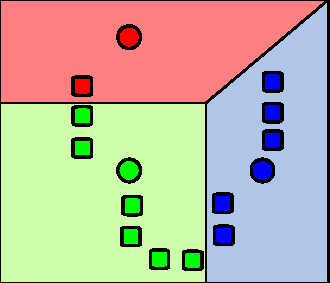
\includegraphics[width=0.15\textwidth]{K_Means_Example_Step_2.pdf}}\\
    \onslide<4->{3. Le centre de chaque classe devient la nouvelle moyenne.} & \\
&\onslide<4->{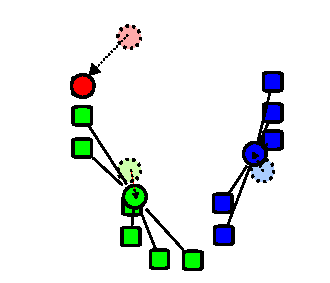
\includegraphics[width=0.15\textwidth]{K_Means_Example_Step_3.pdf}}\\
    \onslide<5->{Les étapes 2 et 3 sont répétées jusqu'à la convergence.} & \\
&\onslide<5->{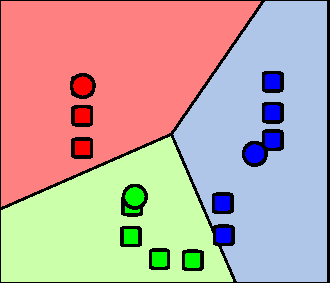
\includegraphics[width=0.15\textwidth]{K_Means_Example_Step_4.pdf}}\\
    \end{tabular}
  \end{center}
{\tiny Images : Wikipedia}
}
\end{frame}

\begin{frame}
\frametitle{Exemple : K-moyennes à 5 classes }
\begin{columns}
\begin{column}{0.5\textwidth}
\begin{figure}[]
  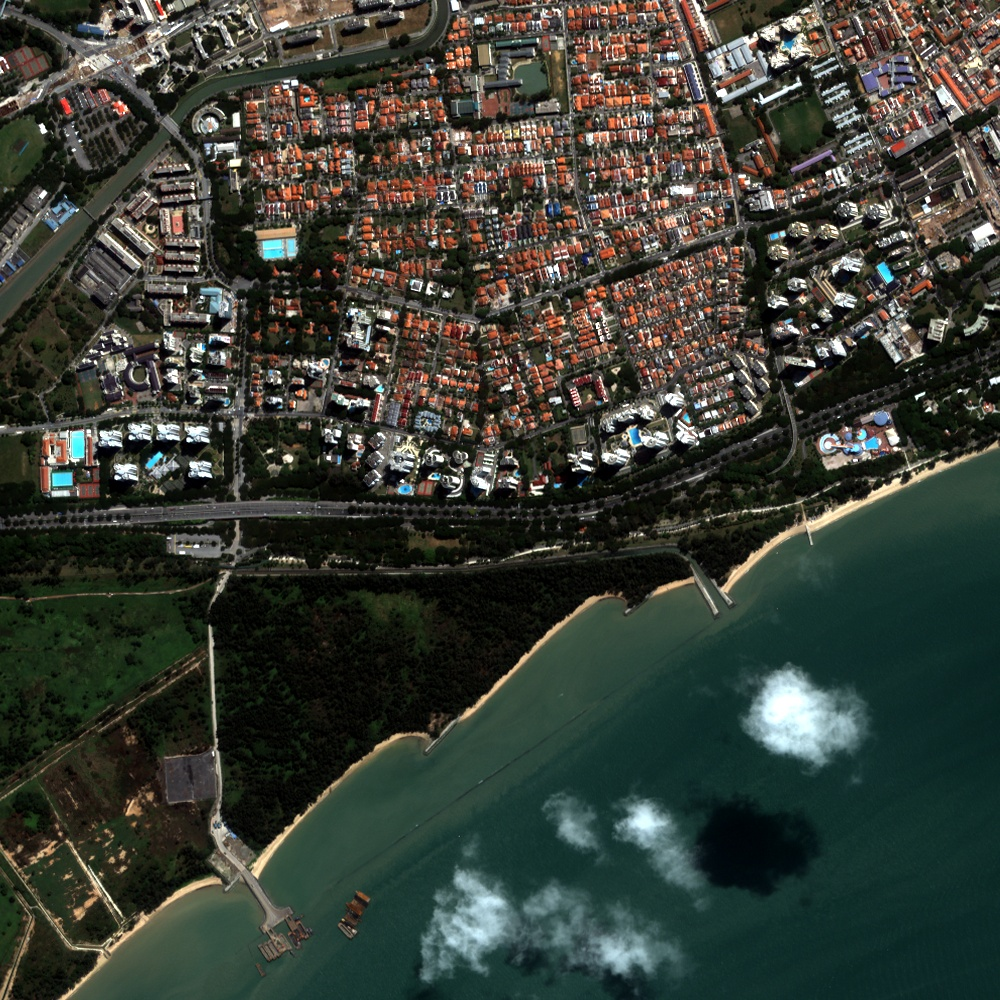
\includegraphics[width=1.0\textwidth]{radio2-extract-3b.jpg}
\end{figure}
\end{column}
\begin{column}{0.5\textwidth}
\begin{figure}[]
  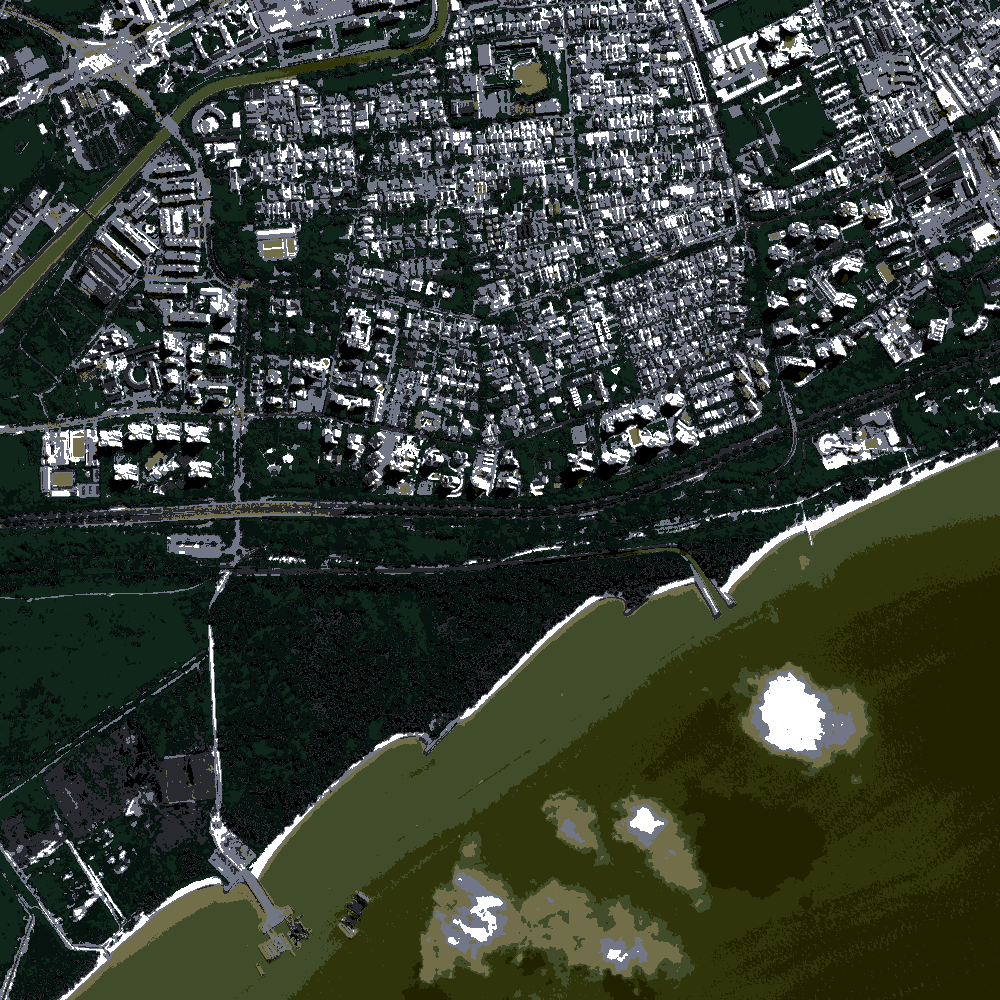
\includegraphics[width=1.0\textwidth]{kmeans-5-classes.png}
\end{figure}
\end{column}
\end{columns}
\end{frame}


\begin{frame}
  \frametitle{La main à la pâte}
  \begin{enumerate}
  \item Monteverdi: Learning $\rightarrow$ KMeans Clustering
  \item Choisir une image
  \item On peut utiliser seulement une fraction des pixels pour
    estimer les centroïdes
  \item Choisir le nombre de classes
  \item Fixer le nombre d'itérations et le seuil de convergence
  \end{enumerate}    
\end{frame}
\section[Supervised]{Classification supervisée}
\label{sec:supervised}
\begin{frame}
  \frametitle{Classification supervisée}
  \begin{itemize}
  \item Nécessite des exemples ou une vérité terrain
  \item Les exemples peuvent avoir des étiquettes thématiques
    \begin{itemize}
    \item Différence entre occupation et utilisation des sols
    \end{itemize}
  \item Exemples: réseaux de neurones, maximum de vraisembkance, Support Vector Machines
  \end{itemize}
\end{frame}

\begin{frame}
  \frametitle{Exemple : SVM}
\setbeamercovered{invisible}
{\tiny
\begin{center}
  \begin{tabular}{cc}
\onslide<2->{H3 (vert) ne sépare pas les 2 classes.} & \onslide<5->{Hyperplan à marge maximale} \\
\onslide<3->{H1 (bleu) OK, mais petite marge.} &  \onslide<5->{SVM appris avec des échantillons de 2 classes.}\\
\onslide<4->{H2 (rouge) marge maximale.} & \onslide<5->{Echantillons
  dans la marge : vecteurs support.}\\
& \\
& \\
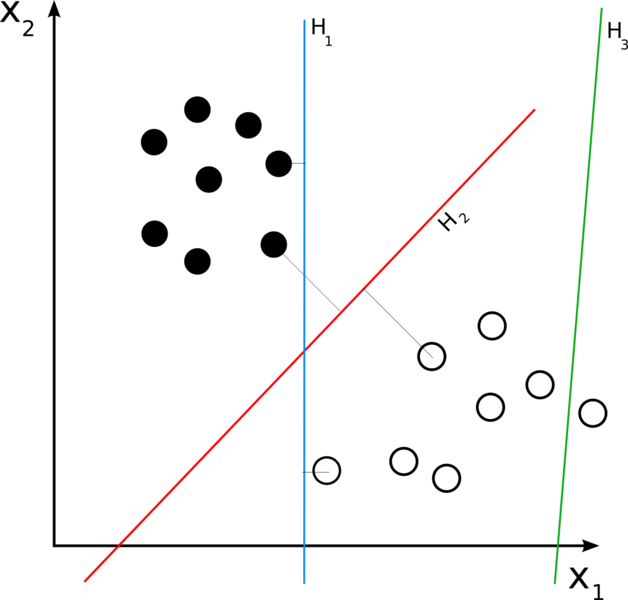
\includegraphics[width=0.3\textwidth]{Svm_separating_hyperplanes.png}
& \onslide<5->{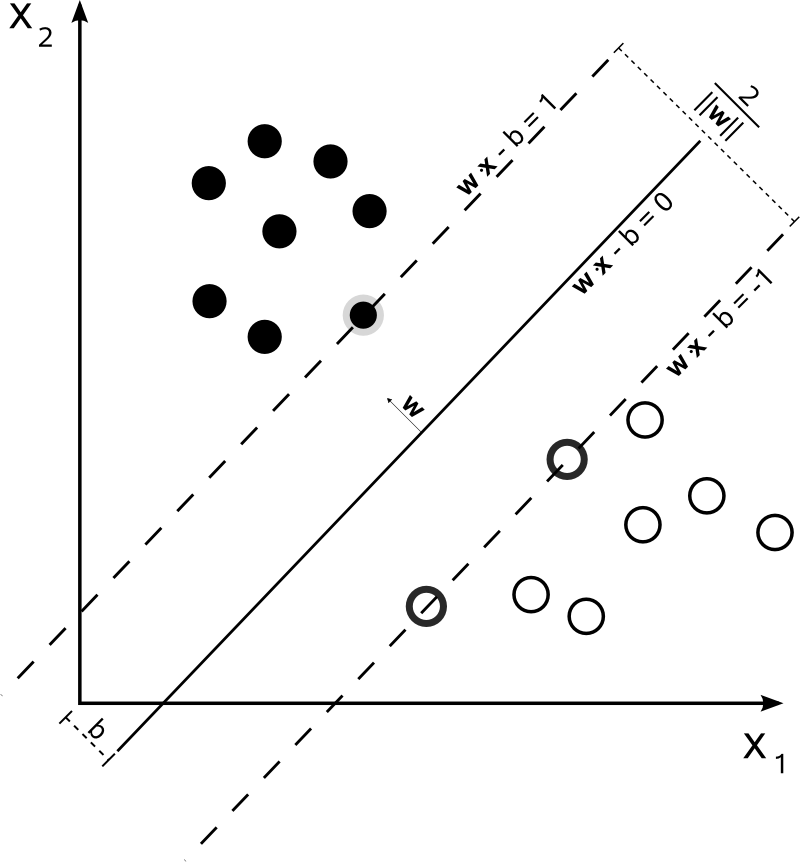
\includegraphics[width=0.3\textwidth]{Svm_max_sep_hyperplane_with_margin.png}}\\
  \end{tabular}
\end{center}
{\tiny Images : Wikipedia}
}
\end{frame}

\begin{frame}
\frametitle{Exemple : SVM à 6 classes}
\framesubtitle{Eau, végétation, bâti, routes, nuages, ombres}
\begin{columns}
\begin{column}{0.5\textwidth}
\begin{figure}[]
  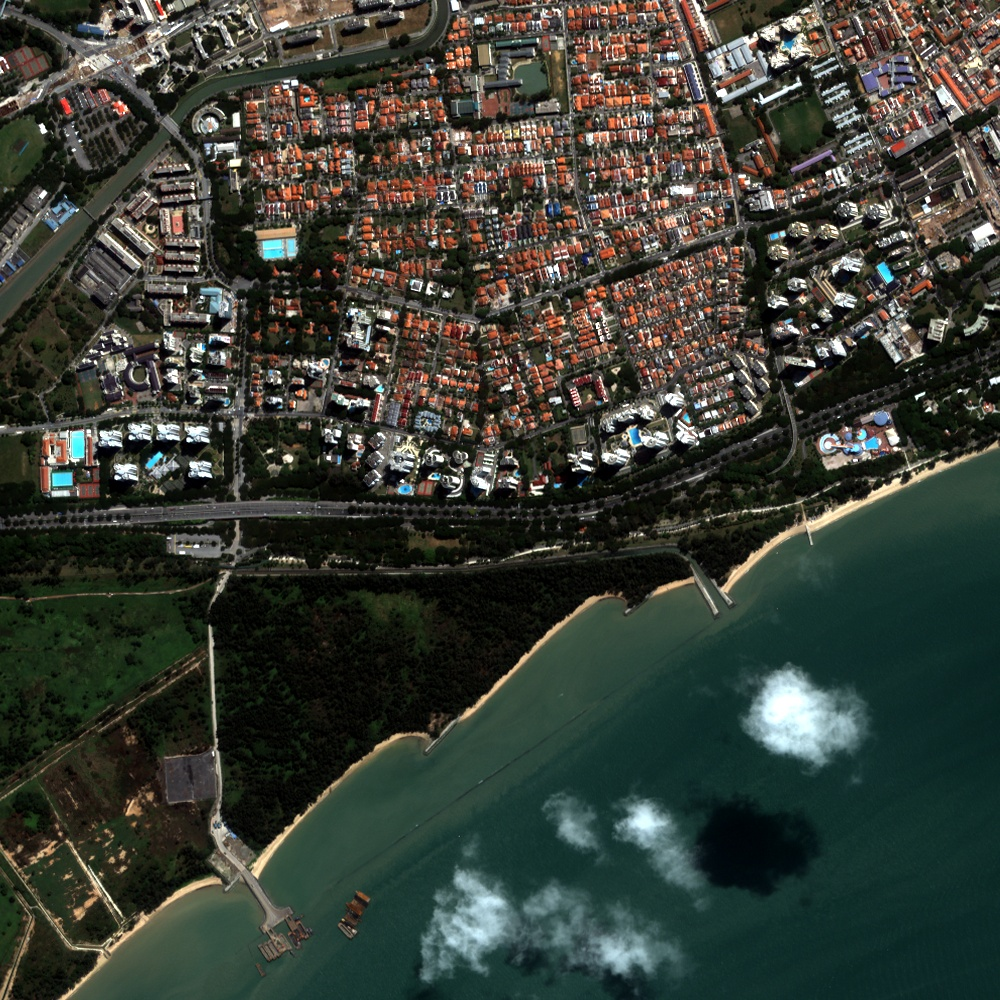
\includegraphics[width=1.0\textwidth]{radio2-extract-3b.jpg}
\end{figure}
\end{column}
\begin{column}{0.5\textwidth}
\begin{figure}[]
  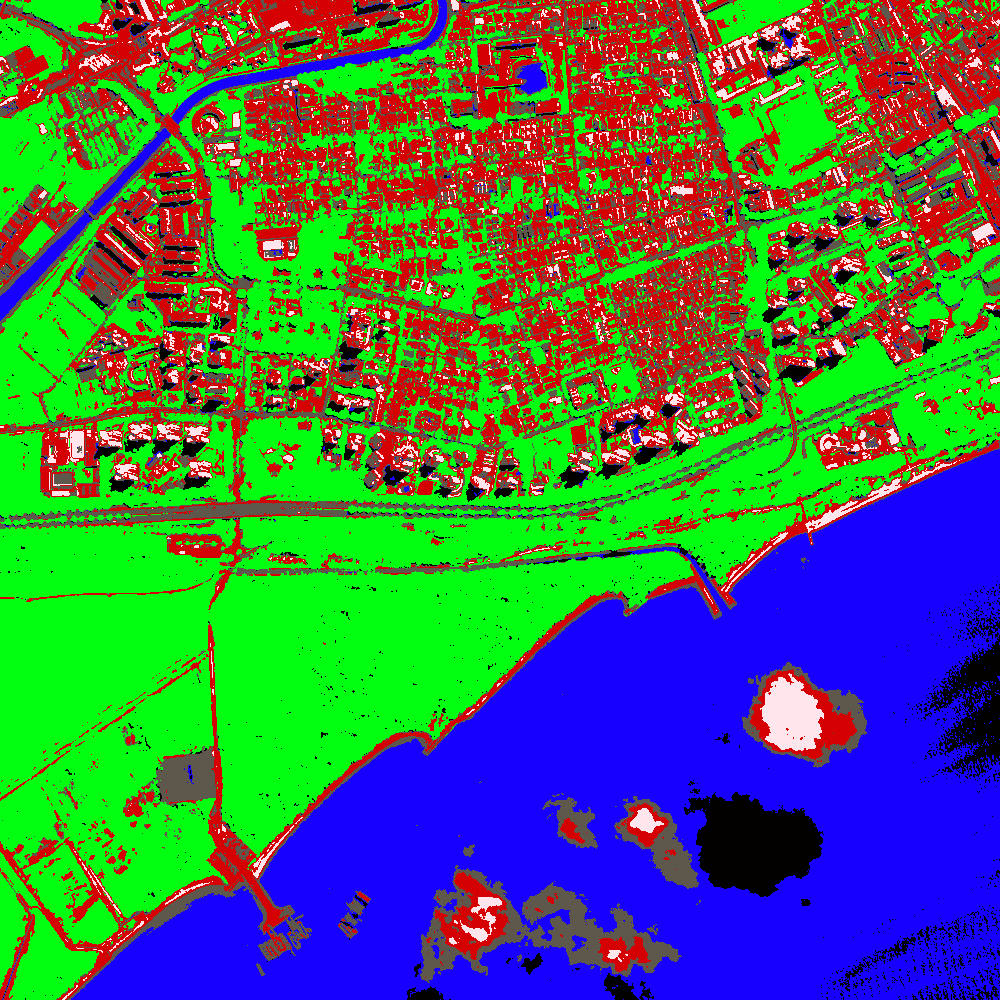
\includegraphics[width=1.0\textwidth]{svm-6-classes.png}
\end{figure}
\end{column}
\end{columns}
\end{frame}


\begin{frame}
  \frametitle{La main à la pâte}
  \begin{enumerate}
  \item Monteverdi: Learning $\rightarrow$ SVM Classification
  \item Choisir l'image à classer
  \item Ajouter une classe
    \begin{itemize}
    \item On peut lui donner un nom et une couleur
    \end{itemize}
  \item Choisir des échantillons pour chaque classe
    \begin{itemize}
    \item Tracer des polygônes et utiliser {\em End Polygon} pour les fermer
    \item On peut associer les polygônes aux ensembles d'apprentissage
      et de test; ou choisir une sélection aléatoire
    \end{itemize}
  \item Learn
  \item Validate : affiche la matrice de confusion
  \item Display : affichage de l'image classée
  \end{enumerate}    
\end{frame}

\section[Object oriented]{Object oriented classification}
\label{sec:objectoriented}
\begin{frame}
  \frametitle{Object oriented classification}
  \begin{itemize}
  \item Pixels may not be the best way to describe the classes of interest
    \begin{itemize}
    \item shape, size, and other region-based characteristics may be
      more meaningful
    \end{itemize}
  \item We need to provide the classifier a set of regions
    \begin{itemize}
    \item Image segmentation
    \end{itemize}
  \item And their characteristics
    \begin{itemize}
    \item Compute features per region 
    \end{itemize}
  \item Since individual objects are meaningful, active learning can
    be implemented
    \begin{itemize}
    \item See presentation WE2.L06.2 {\em ``LAZY YET EFFICIENT LAND-COVER
      MAP GENERATION FOR HR OPTICAL IMAGES''}, Wednesday, July 28, 10:25
    - 12:05, by Julien Michel, Julien Malik and Jordi Inglada.
    \end{itemize}
  \end{itemize}
\end{frame}

\begin{frame}
  \frametitle{No hands on}
But a demo if the time allows it!
\end{frame}


\end{document}
